\documentclass[a4paper,11pt]{ltjsarticle}
\usepackage[margin=25mm]{geometry}
\usepackage{amsmath,listings,enumitem,booktabs,longtable,multirow,tikz,float,caption}
\captionsetup{font=small}
\lstset{basicstyle=\small\ttfamily,numbers=left,frame=single}
\begin{document}
\tableofcontents
\clearpage
\section{窓札の観察}
\noindent MarkA 本文を二行写す。\\
MarkB 次の紙片を読む。
\begin{center}透明な窓札\\細い刻み\end{center}
\noindent MarkC 隣の台を調べる。
\begin{quote}窓の左端を揃える。\\同じ長さの札を二組作る。\end{quote}
\noindent MarkD 青い行を写す。
\begin{verse}浅い窓の印\\深い窓の印

西側の窓の印\end{verse}
\noindent MarkE 紙を数える。
\begin{itemize}[itemsep=3pt]
\item 白い札
\begin{itemize}\item 細い窓\item 広い窓\end{itemize}
\item 黄色い札
\end{itemize}
\noindent MarkF 裏の印を確かめる。
\begin{enumerate}\item 外側を測る。\item 裏返す。\item 数値を記す。\end{enumerate}
\noindent MarkG 長さを比べる。
\begin{description}[style=nextline,leftmargin=4em,labelwidth=3em]
\item[端] 短い方。
\item[折り返した場所] 二枚を重ねた位置。
\end{description}
\noindent MarkH 控えを残す。
\clearpage
\section{集計の手順}
\noindent MarkI 枚数を写す。
\begin{lstlisting}[caption={窓札を数える}]
thin = 2
wide = 4
total = thin + wide
\end{lstlisting}
\noindent MarkJ 表に結果を記す。
\begin{table}[H]\centering
\caption{二組の窓札}
\begin{tabular}{lcr}\toprule
形 & 場所 & 数 \\ \midrule
\multirow{2}{*}{細長} & 東 & 2 \\ & 西 & 5 \\
正方 & 南 & 4 \\ \bottomrule
\end{tabular}
\end{table}
\noindent MarkK 図を控える。
\begin{figure}[H]\centering
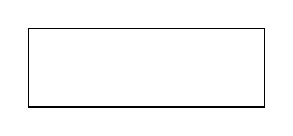
\begin{tikzpicture}\draw (0,0) rectangle (3,1);\end{tikzpicture}
\caption{外側の札。\\裏側からも同じ形に見える。}
\end{figure}
\noindent MarkL 次の列を照合する。
\begin{longtable}{lr}\toprule 札 & 数 \\ \midrule
狭い窓 & 3 \\ 広い窓 & 4 \\ 丸い窓 & 2 \\ \bottomrule
\end{longtable}
\noindent MarkM 作業を終える。
\clearpage
\appendix
\section{台の見取図}
\subsection{折り目の位置}
\noindent MarkN 左右の台を用意する。
\par\noindent\begin{minipage}[t]{.46\linewidth}
\subsubsection*{左の台}狭い窓の札。\\二枚重ねる。
\end{minipage}\hfill
\begin{minipage}[t]{.46\linewidth}
\subsubsection*{右の台}広い窓の札。\\一枚広げる。
\end{minipage}\par
\noindent MarkO 幅を記す。
\[ a = 27 \]
\noindent MarkP 縁の長さを記す。
\begin{align*} b &= a+2 \\ c &= b+3 \end{align*}
\noindent MarkQ 参照票を閉じる。
\begin{thebibliography}{9}
\bibitem{narrow} MarkR 窓札工房『紙の幅』。
\bibitem{wide} MarkS 砂板室『丸い縁』。
\bibitem{fold} MarkT 折り箱室『輪の控え』。
\end{thebibliography}
\noindent MarkU 終端の印。
\end{document}
